\documentclass{exam}
\usepackage[utf8]{inputenc}

\usepackage[dvipsnames]{xcolor}
\usepackage{microtype}
\usepackage{siunitx}
\DeclareSIUnit\year{yr}
\usepackage{pgfplots}
\usepackage{graphicx}
\usepackage{float}
\usepackage{hyperref}

\renewcommand*{\thefootnote}{\fnsymbol{footnote}}


\begin{document}

\section*{NCEA Level 1 Science (Genetics \#3)}

This worksheet is on reproduction and variation.

\subsection*{Questions}
\begin{questions}
  \question Explain why variation is advantageous for a species over time.
  \question {[NZQA 2015]} The photograph below shows a large number of plants that are all the same species.
            \begin{center}
              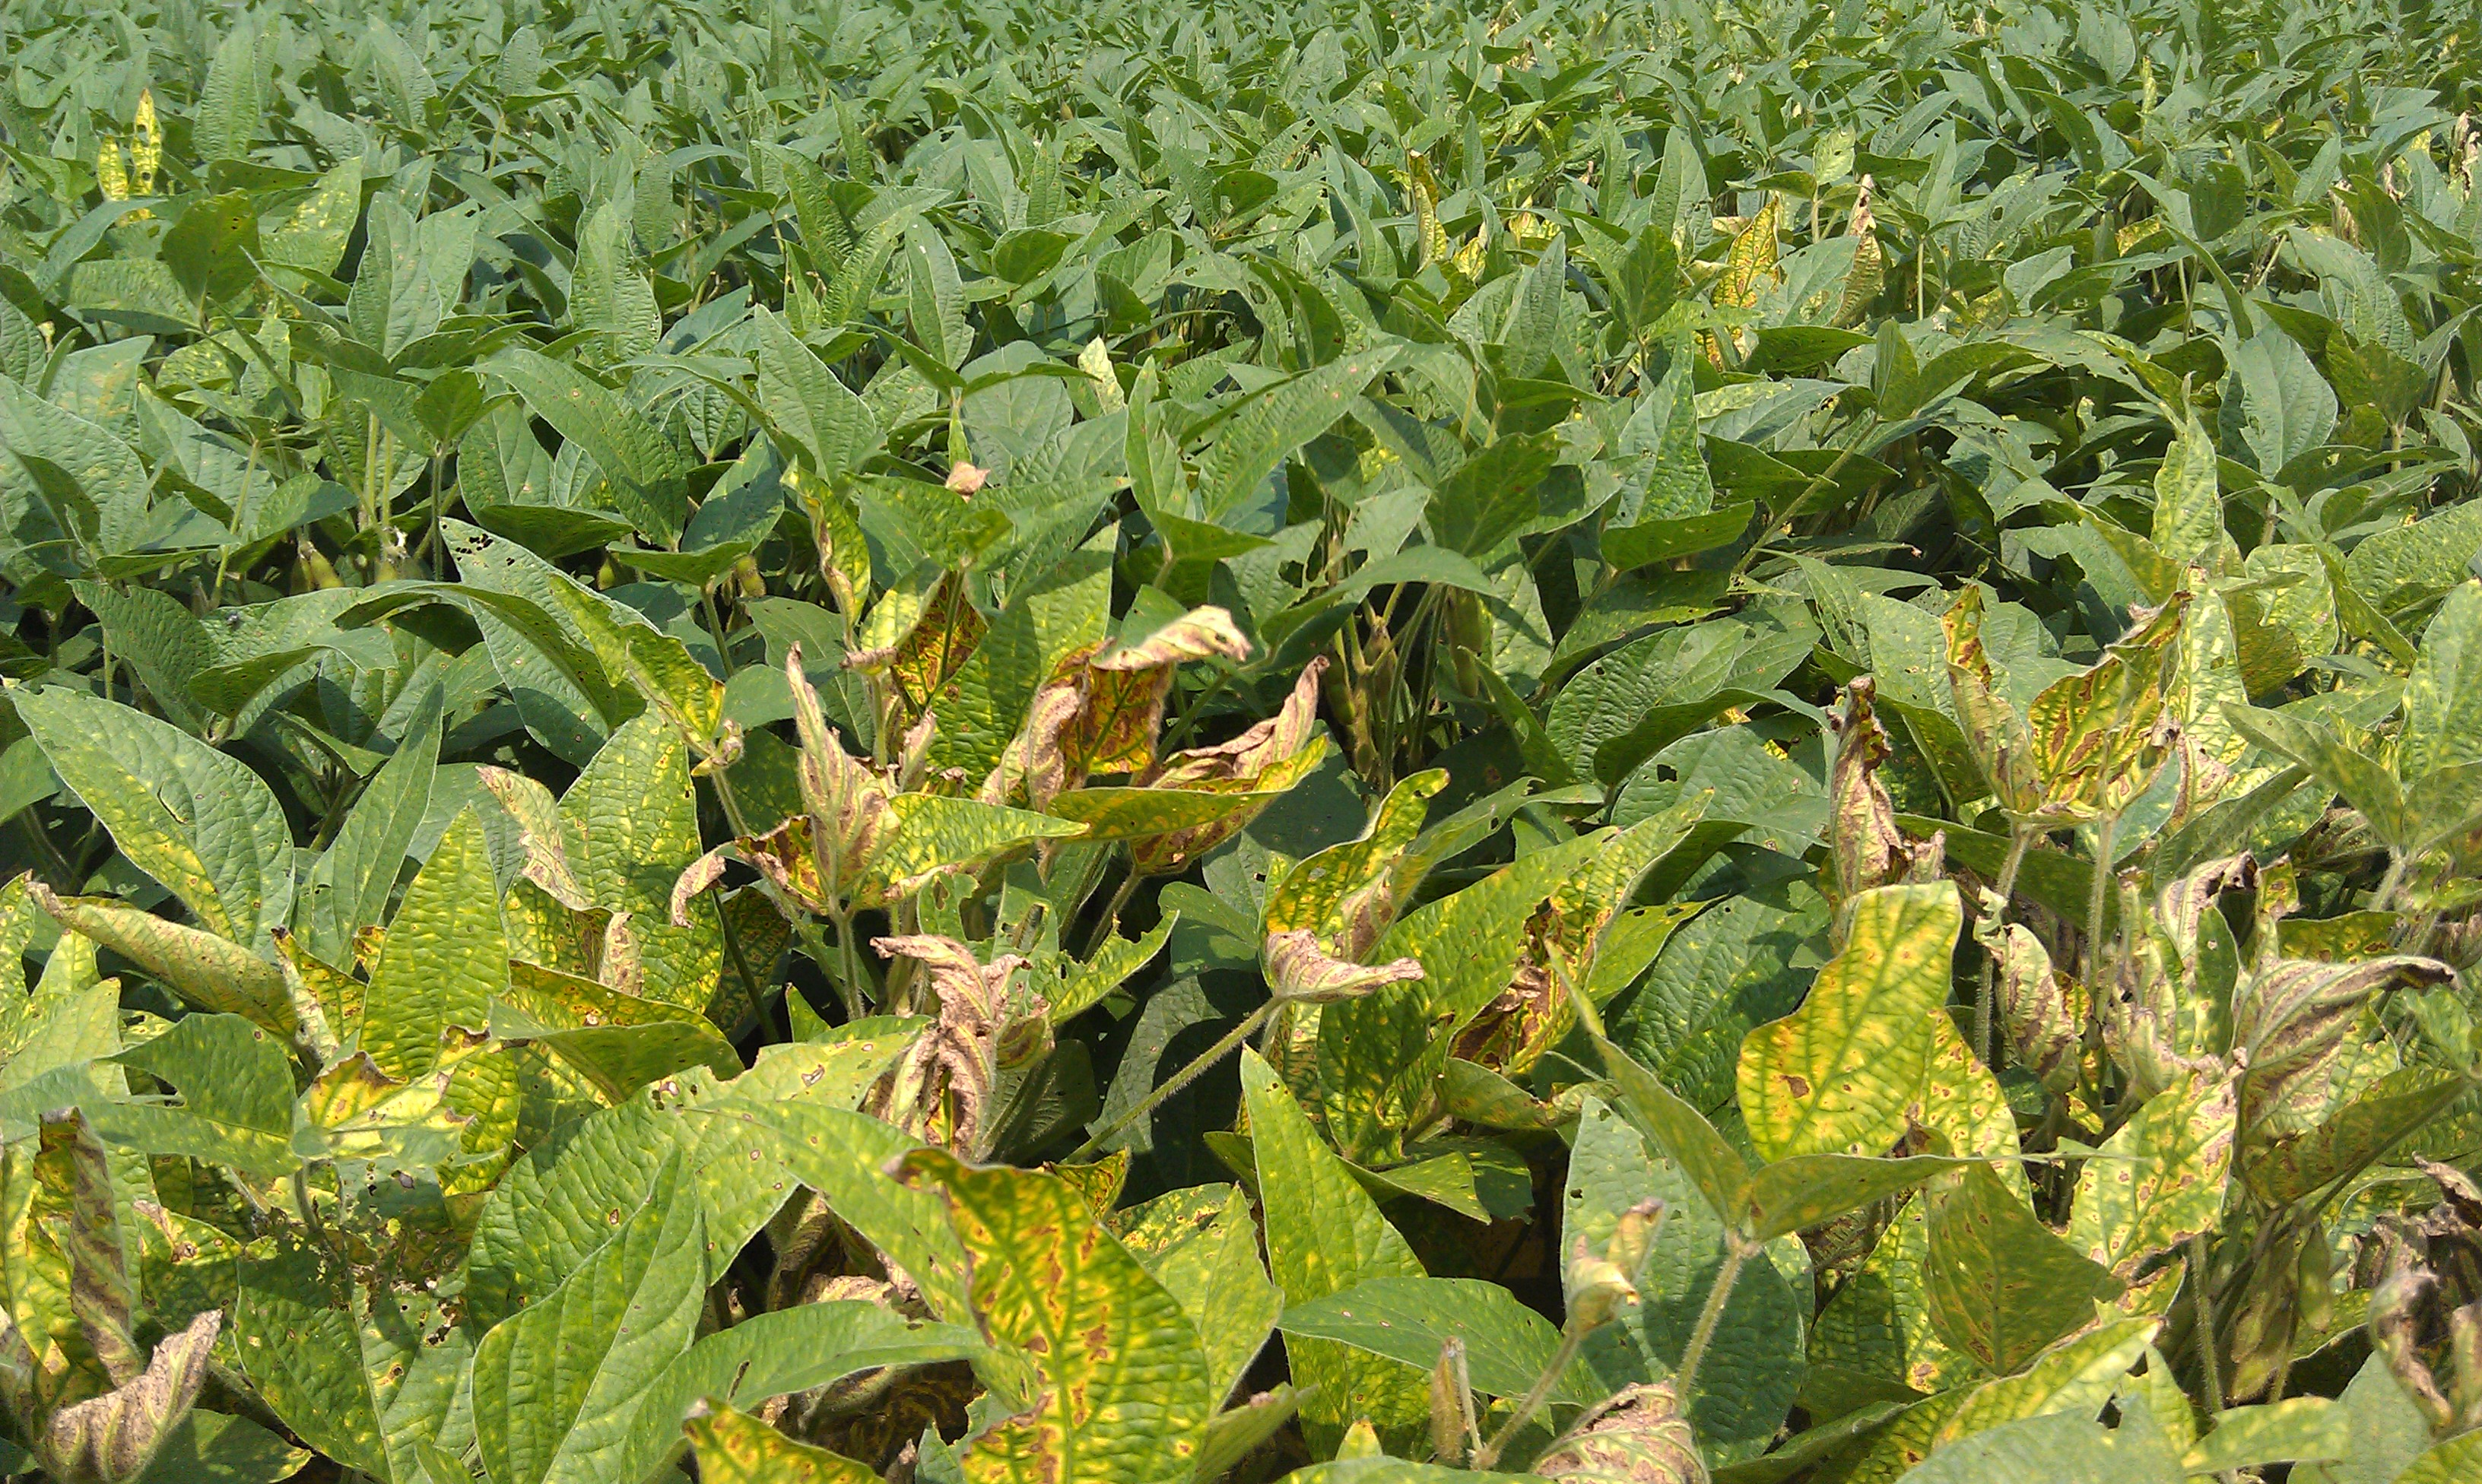
\includegraphics[width=0.7\textwidth]{stemrot}
            \end{center}
    \begin{parts}
      \part The yellow-brown colour in some of the plants has been caused by a disease. The disease is present throughout the field, but affects
            only some plants. This is because of variation in the plants. Explain why variation means not all the plants get the disease.
      \part The plants in the photograph were grown from seeds. Seeds are the result of sexual reproduction.
        \begin{subparts}
          \subpart Name one process that occurs during sexual reproduction, and explain how it results in variation.
          \subpart Discuss the advantages of sexual reproduction for a species when the environment changes. In your answer you should:
            \begin{itemize}
              \item give examples of a changing environment
              \item explain the impact of changing environments on a population
              \item consider the importance of variation in a population in a changing environment.
            \end{itemize}
        \end{subparts}
    \end{parts}
  \question {[NZQA 2017]} Wild bananas have large seeds, and reproduce sexually. Farmed bananas are produced asexually, from suckers called “banana pups”.
    \begin{parts}
      \part How does the production of gametes by the wild banana plants result in variation?
      \part Suggest what possible problems may arise for the asexually produced farmed plants that do not arise for the wild plants.
    \end{parts}
  \question ``Pseudomonas syringae pv. actinidiae (Psa) is a bacteria that can result in the death of kiwifruit vines. It was first discovered in
            New Zealand in November 2010 and rapidly caused widespread and severe impacts to New Zealand's kiwifruit industry.

            ``New genetic material of any strain is a concern due to the potential of horizontal gene transfer and the impact new strains may have
            on new or existing kiwifruit cultivars.

            ``New strains of Psa are also expected to evolve within New Zealand, of which the characteristics and virulence to new and existing
            kiwifruit cultivars are unknown. Good biosecurity practices are vital to prevent the spread of any new strains between orchards and
            growing regions.''\footnote{~\url{http://www.kvh.org.nz/about_psa}}

            Discuss why biological threats to New Zealand plants, like the Psa virus, tend to affect cultivated species rather than wild species.

            In your answer, you should (with reference to the example above):
            \begin{itemize}
              \item Describe how cultivated plants are reproduced, and contrast this to the reproduction of wild plants.
              \item Explain how this difference makes cultivated plants more susceptible to diseases.
              \item Guess the meaning of `horizontal gene transfer' with respect to the bacteria involved, and explain why it is advantageous for the
                    bacteria species. [Hint: normal sexual reproduction results in \emph{vertical} gene transfer.]
            \end{itemize}
\end{questions}

\subsection*{Homework}
\begin{questions}
  \question {[NZQA 2012]} The diagram below shows the relationship between chromosomes, genes, and DNA (deoxyribonucleic acid).
            \begin{center}
              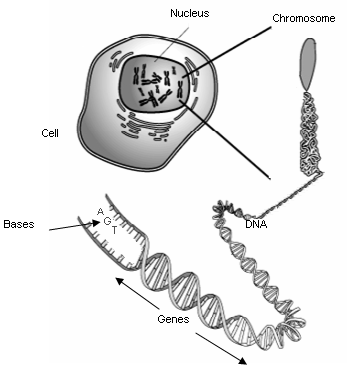
\includegraphics[width=0.5\textwidth]{dnadiagram}
            \end{center}
    \begin{parts}
      \part Explain the relationships between DNA, chromosomes and genes. You may add notes and labels to the diagram above to support your answer.
      \part Explain how the relationships in your answer to (a) lead to different characteristics and how this contributes to genetic variation.
    \end{parts}
  \question {[NZQA 2012]} A blood disorder caused by red blood cells with an unusual curved (sickle) shape is inherited through a single gene with
            two possible alleles, normal and sickle.

            Use `H' to represent the dominant `normal' allele, and `h' to represent the recessive `sickle' allele.
    \begin{parts}
      \part Explain how two parents with normal blood cells can have a child with sickle-shaped blood cells, with reference to the genotypes of \textbf{both}
            normal parents and a child with sickle-shaped blood cells. You may refer to a Punnett square in your answer.
      \part The parents in part (a) have four children all with sickle-shaped blood cells. They are expecting a fifth child. Explain how normal parents
            could have produced \textbf{four} children with sickle-shaped blood cells, and calculate the chance that the fifth child will also have sickle-shaped
            blood cells.
    \end{parts}
\end{questions}

\end{document}
